\documentclass[aspectratio=169,10pt]{beamer}

% ---- Engine / fonts -------------------------------------------------
\usepackage{fontspec}
\setsansfont{Liberation Sans}
\setmonofont{DejaVu Sans Mono}[Scale=0.85]

\usepackage{xeCJK}
\setCJKmainfont{Noto Sans CJK KR}
\setCJKsansfont{Noto Sans CJK KR}

% ---- Packages -------------------------------------------------------
\usepackage{xcolor}
\usepackage{booktabs}
\usepackage{array}
\usepackage{tikz}
\usetikzlibrary{arrows.meta, positioning, shapes.geometric, backgrounds, calc}
\usepackage{tcolorbox}
\tcbuselibrary{skins, breakable}
\usepackage{amsmath, amssymb}

% ---- Palette (matches week09) ---------------------------------------
\definecolor{slate}{HTML}{4B586B}
\definecolor{slatedark}{HTML}{3A4554}
\definecolor{slatelight}{HTML}{7A8699}
\definecolor{coral}{HTML}{C97865}
\definecolor{corallight}{HTML}{F1DED7}
\definecolor{greenpos}{HTML}{7FA06B}
\definecolor{greenposlight}{HTML}{DFE8D2}
\definecolor{bluesoft}{HTML}{8AA5C2}
\definecolor{bluesoftlight}{HTML}{DCE4EE}
\definecolor{rulegrey}{HTML}{B8BFCA}

% ---- Beamer theme (custom) -----------------------------------------
\setbeamercolor{normal text}{fg=slatedark, bg=white}
\setbeamercolor{structure}{fg=slate}
\setbeamercolor{frametitle}{fg=slate, bg=white}
\setbeamercolor{framesubtitle}{fg=slatelight, bg=white}
\setbeamercolor{title}{fg=white, bg=slate}
\setbeamercolor{author}{fg=slatedark}
\setbeamercolor{institute}{fg=slatelight}
\setbeamercolor{date}{fg=slatelight}
\setbeamercolor{itemize item}{fg=slate}
\setbeamercolor{itemize subitem}{fg=slate}
\setbeamercolor{enumerate item}{fg=coral}

\setbeamerfont{frametitle}{size=\Large, series=\bfseries}
\setbeamerfont{framesubtitle}{size=\small, series=\bfseries}
\setbeamerfont{title}{size=\LARGE, series=\bfseries}
\setbeamerfont{subtitle}{size=\large, series=\bfseries}
\setbeamerfont{author}{size=\normalsize}
\setbeamerfont{institute}{size=\small}
\setbeamerfont{date}{size=\small}

\setbeamertemplate{itemize item}{\raisebox{0.25ex}{\rule{4pt}{4pt}}}
\setbeamertemplate{itemize subitem}{\raisebox{0.35ex}{\rule{3pt}{3pt}}}
\setbeamertemplate{navigation symbols}{}

% Frametitle with coral rule below
\setbeamertemplate{frametitle}{%
  \nointerlineskip
  \vspace*{0.8em}
  \begin{beamercolorbox}[wd=\paperwidth, leftskip=1.1em, rightskip=1em]{frametitle}%
    \usebeamerfont{frametitle}\insertframetitle\par
    \ifx\insertframesubtitle\@empty\else
      \vspace{0.15em}\usebeamerfont{framesubtitle}\usebeamercolor[fg]{framesubtitle}\insertframesubtitle\par
    \fi
    \vspace{0.25em}
    {\color{coral}\rule{\dimexpr\paperwidth-2.1em\relax}{0.8pt}}%
  \end{beamercolorbox}%
  \vspace*{0.3em}
}

% Footline: course title left, page / total right
\setbeamertemplate{footline}{%
  \leavevmode%
  \hbox to \paperwidth{%
    \hspace*{1.1em}{\scriptsize\color{slatelight}BA2: Digital Korea}%
    \hfill%
    {\scriptsize\color{slatelight}\insertframenumber\,/\,\inserttotalframenumber}%
    \hspace*{1.1em}%
  }%
  \vspace{0.7em}%
}

% Title page
\setbeamertemplate{title page}{%
  \vfill
  \begin{beamercolorbox}[wd=0.9\paperwidth, center, rounded=true, shadow=true, sep=1.2em]{title}%
    \usebeamerfont{title}\inserttitle\par
    \vspace{0.4em}
    {\usebeamerfont{subtitle}\color{white!85}\insertsubtitle}
  \end{beamercolorbox}%
  \vfill
  \begin{center}
    {\usebeamerfont{author}\color{slatedark}\insertauthor\par}
    \vspace{0.6em}
    {\usebeamerfont{institute}\color{slatelight}\insertinstitute\par}
    \vspace{1.2em}
    {\usebeamerfont{date}\color{slatelight}\insertdate}
  \end{center}
  \vfill
}

% Section title (big centered text + coral rule)
\AtBeginSection[]{%
  \begin{frame}[plain, noframenumbering]
    \vfill
    \centering
    {\color{slate}\fontsize{32pt}{38pt}\selectfont\bfseries\insertsection\par}
    \vspace{0.6em}
    {\color{coral}\rule{0.22\paperwidth}{0.6pt}}
    \vfill
  \end{frame}%
}

% ---- Callout-box helpers -------------------------------------------
\newtcolorbox{callcoral}[1][]{%
  enhanced, breakable, sharp corners,
  colback=corallight, colframe=corallight,
  coltitle=white, colbacktitle=coral,
  fonttitle=\bfseries,
  title={#1},
  left=1em, right=1em, top=0.5em, bottom=0.6em,
  boxrule=0pt, titlerule=0pt,
}
\newtcolorbox{callblue}[1][]{%
  enhanced, breakable, sharp corners,
  colback=bluesoftlight, colframe=bluesoftlight,
  coltitle=white, colbacktitle=bluesoft,
  fonttitle=\bfseries,
  title={#1},
  left=1em, right=1em, top=0.5em, bottom=0.6em,
  boxrule=0pt, titlerule=0pt,
}

% Little token boxes (for inline diagrams)
\newcommand{\tokbox}[2][bluesoftlight]{%
  \tikz[baseline=(N.base)]\node[draw=slatelight, rounded corners=2pt,
        fill=#1, inner sep=3pt, font=\small] (N) {#2};%
}
\newcommand{\poschip}[1]{%
  \tikz[baseline=(N.base)]\node[draw=greenpos, rounded corners=2pt,
        fill=greenposlight, inner sep=3pt, font=\small] (N) {#1};%
}
\newcommand{\negchip}[1]{%
  \tikz[baseline=(N.base)]\node[draw=coral, rounded corners=2pt,
        fill=corallight, inner sep=3pt, font=\small] (N) {#1};%
}

% ---- Meta -----------------------------------------------------------
\title{BA2: Digital Korea}
\subtitle{Week 10: Topic Modeling (LDA)}
\author{Steven Denney}
\institute{Korean Studies\\Leiden University}
\date{April 20, 2026}

\begin{document}

% ==================================================================
\begin{frame}[plain, noframenumbering]
  \titlepage
\end{frame}

% ------------------------------------------------------------------
\begin{frame}{Today's Agenda}
  \begin{enumerate}
    \item Review \& check-in: from feeling to theme
    \item What is topic modeling?
    \item LDA: the intuition
    \item Choosing $k$ (the number of topics)
    \item Orange's Topic Modelling widget under the hood
    \item Application: the NIKH Korean history textbook corpus
    \item Interpreting topics responsibly
    \item Looking ahead
  \end{enumerate}
\end{frame}

% ==================================================================
\section{Review \& Check-In}

\begin{frame}{From Feeling to Theme}{Week 9 asked \emph{how} a text feels; Week 10 asks \emph{what} it is about}
  \textbf{Last week (sentiment):} each text gets \emph{one number} --- a tone.
  \begin{center}
    \poschip{감사} \; $+$ \; \poschip{희망} \; $+$ \; \negchip{위기} \; $\Rightarrow$ \; a positive/negative \emph{score}
  \end{center}

  \vspace{0.6em}
  \textbf{This week (topics):} each text gets \emph{several numbers} --- a mixture of themes.
  \begin{center}
    \emph{One textbook} \; $\Rightarrow$ \;
    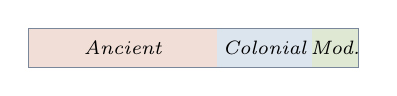
\begin{tikzpicture}[baseline={(0,0.15)}]
      \fill[corallight]    (0,0)   rectangle (2.4,0.5);
      \fill[bluesoftlight] (2.4,0) rectangle (3.6,0.5);
      \fill[greenposlight] (3.6,0) rectangle (4.2,0.5);
      \draw[slatelight, thin] (0,0) rectangle (4.2,0.5);
      \node[font=\scriptsize\itshape] at (1.2,0.25) {Ancient};
      \node[font=\scriptsize\itshape] at (3.0,0.25) {Colonial};
      \node[font=\scriptsize\itshape] at (3.9,0.25) {Mod.};
    \end{tikzpicture}
  \end{center}

  \vspace{0.4em}
  \emph{Sentiment:} \textbf{how} does the text feel? \\
  \emph{Topics:} \textbf{what} themes run through this collection of texts?
\end{frame}

\begin{frame}{Warm-up in English}{Shout out a label for each list --- no wrong answers}
  \vspace{0.3em}

  \textbf{1.} \quad \tokbox{kimchi} \; \tokbox{bulgogi} \; \tokbox{ramyeon} \; \tokbox{soju} \; \tokbox{rice} \; \tokbox{banchan}
  \vspace{0.4em}

  \textbf{2.} \quad \tokbox{BTS} \; \tokbox{idol} \; \tokbox{fandom} \; \tokbox{album} \; \tokbox{stage} \; \tokbox{concert}
  \vspace{0.4em}

  \textbf{3.} \quad \tokbox{king} \; \tokbox{palace} \; \tokbox{scholar} \; \tokbox{dynasty} \; \tokbox{robe} \; \tokbox{sword}
  \vspace{0.4em}

  \textbf{4.} \quad \tokbox{subway} \; \tokbox{cafe} \; \tokbox{apartment} \; \tokbox{delivery} \; \tokbox{convenience} \; \tokbox{night}
\end{frame}

\begin{frame}{What You Just Did}{Six words in, a theme out --- that is the topic-modeling move}
  \vspace{0.4em}
  \begin{center}
    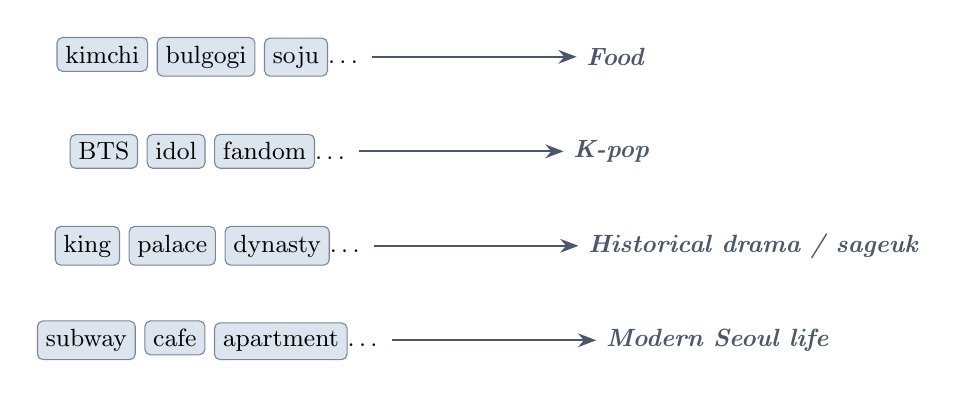
\begin{tikzpicture}[
      every node/.style={font=\small},
      wordlist/.style={font=\small, align=left},
      arr/.style={-Stealth, thick, slate},
      label/.style={font=\small\bfseries, text=slate, align=left},
    ]
      \node[wordlist] (l1) at (0,2.4) {\tokbox{kimchi} \tokbox{bulgogi} \tokbox{soju}\ldots};
      \node[wordlist] (l2) at (0,1.2) {\tokbox{BTS} \tokbox{idol} \tokbox{fandom}\ldots};
      \node[wordlist] (l3) at (0,0)   {\tokbox{king} \tokbox{palace} \tokbox{dynasty}\ldots};
      \node[wordlist] (l4) at (0,-1.2){\tokbox{subway} \tokbox{cafe} \tokbox{apartment}\ldots};

      \node[label, right=2.6cm of l1] (t1) {\textit{Food}};
      \node[label, right=2.6cm of l2] (t2) {\textit{K-pop}};
      \node[label, right=2.6cm of l3] (t3) {\textit{Historical drama / sageuk}};
      \node[label, right=2.6cm of l4] (t4) {\textit{Modern Seoul life}};

      \draw[arr] (l1.east) -- (t1.west);
      \draw[arr] (l2.east) -- (t2.west);
      \draw[arr] (l3.east) -- (t3.west);
      \draw[arr] (l4.east) -- (t4.west);
    \end{tikzpicture}
  \end{center}

  \vspace{0.3em}
  \begin{callblue}[What you just did]
    You read six co-occurring words and inferred a theme. LDA does the opposite direction:
    it reads a corpus and returns lists like the ones on the left, for \emph{you} to label.
  \end{callblue}
\end{frame}

\begin{frame}{Now in Korean}{Same game --- each list is the top six words of one topic}
  \vspace{0.3em}

  \textbf{1.} \quad \tokbox{고구려} \; \tokbox{백제} \; \tokbox{신라} \; \tokbox{삼국} \; \tokbox{왕} \; \tokbox{시대}
  \vspace{0.4em}

  \textbf{2.} \quad \tokbox{일제} \; \tokbox{독립} \; \tokbox{저항} \; \tokbox{운동} \; \tokbox{항일} \; \tokbox{식민}
  \vspace{0.4em}

  \textbf{3.} \quad \tokbox{경제} \; \tokbox{산업화} \; \tokbox{발전} \; \tokbox{성장} \; \tokbox{정부} \; \tokbox{수출}
  \vspace{0.4em}

  \textbf{4.} \quad \tokbox{민족} \; \tokbox{정체성} \; \tokbox{민주} \; \tokbox{시민} \; \tokbox{통일} \; \tokbox{문화}

  \vspace{0.9em}
  \begin{callblue}[Discuss with a neighbour]
    What label fits each list? Are any two close to each other?
  \end{callblue}
\end{frame}

\begin{frame}{Now in Korean: Answers}{Plausible labels for the Korean lists}
  \vspace{0.1em}
  \begin{center}
    \small
    \begin{tabular}{@{}c l l@{}}
      \toprule
      \textbf{\#} & \textbf{Top words} & \textbf{A plausible label} \\
      \midrule
      1 & 고구려, 백제, 신라, 삼국, 왕, 시대 & Ancient \& Three Kingdoms \\
      2 & 일제, 독립, 저항, 운동, 항일, 식민 & Colonial era / resistance \\
      3 & 경제, 산업화, 발전, 성장, 정부, 수출 & Modernisation \\
      4 & 민족, 정체성, 민주, 시민, 통일, 문화 & Modern Korean identity \\
      \bottomrule
    \end{tabular}
  \end{center}

  \vspace{0.5em}
  \begin{callcoral}[The takeaway]
    This \emph{is} what LDA produces: ranked lists of words. The \textbf{model} finds co-occurring words;
    \textbf{you} read them and assign the label. Labels are interpretations, not facts ---
    a list about \emph{nation}, \emph{democracy}, \emph{citizenship}, \emph{identity} could plausibly be read two ways.
  \end{callcoral}
\end{frame}

\begin{frame}{Where LDA Fits Among Our Methods}{Each method gives a different \emph{kind} of answer about a document}
  \begin{center}
    \small
    \begin{tabular}{@{}c l l@{}}
      \toprule
      \textbf{Week} & \textbf{Method}              & \textbf{What each document gets} \\
      \midrule
      7    & Clustering (K-means, hierarchical)   & \emph{one} group (a hard label)               \\
      8    & Word embeddings                      & a vector --- a position in meaning space       \\
      9    & Dictionary sentiment                 & \emph{one} score (a tone)                      \\
      \textbf{10} & \textbf{LDA (topic modeling)} & \textbf{a \emph{mixture} over themes (many weights)} \\
      \bottomrule
    \end{tabular}
  \end{center}

  \vspace{0.8em}
  Clustering and sentiment each give a \emph{single} answer per document. Embeddings give a fixed representation.\\
  \textbf{LDA is the first method that gives each document a \emph{multi-valued} answer} ---
  a document isn't one thing, it is a blend of several, in different proportions.
\end{frame}

% ==================================================================
\section{What Is Topic Modeling?}

\begin{frame}{From a Sea of Text to Hidden Structure}{The problem: corpora too big to read, too important to ignore}
  \begin{itemize}
    \item The NIKH corpus we will use today covers \textbf{67 Korean history textbooks} (1895--2016).
    \item Even the 11-book demo already runs past a \emph{million characters of Korean prose}.
    \item You cannot close-read it all. You also cannot reduce it to a single number.
  \end{itemize}
  \vspace{0.4em}
  \begin{callblue}[The topic modeling question]
    What \textbf{themes} run through this collection, \textbf{how much} does each document use each theme,
    and \textbf{which words} define each theme?
  \end{callblue}
\end{frame}

\begin{frame}{Topic Modeling: The Basic Idea}{An unsupervised method for discovering hidden thematic structure}
  \begin{itemize}
    \item A \textbf{topic} is a group of words that tend to appear together across the corpus.
    \item Each \textbf{document} is represented as a \textbf{mixture of topics}.
    \item The algorithm does not know, in advance, what the topics are. It \emph{discovers} them.
  \end{itemize}

  \vspace{0.6em}
  Topic modeling answers three questions:
  \begin{enumerate}
    \item What themes appear across the documents?
    \item How much of each theme does a given document contain?
    \item Which words \emph{define} each theme?
  \end{enumerate}
\end{frame}

% ==================================================================
\section{How LDA Works}

\begin{frame}{Latent Dirichlet Allocation, in Plain Words}{The most widely used topic model; Orange runs it}
  LDA (Blei, Ng \& Jordan, 2003) makes two simple assumptions:
  \begin{enumerate}
    \item Each \textbf{document} is made up of several \textbf{topics}, in some proportion.
    \item Each \textbf{topic} is made up of \textbf{words that tend to occur together}.
  \end{enumerate}

  \vspace{0.4em}
  It reads a corpus as a \textbf{term--document matrix of word counts} --- a bag of words, not TF--IDF weights.

  \vspace{0.4em}
  \emph{Latent} --- the topics are hidden; we only observe words.\\
  \emph{Dirichlet} --- a statistical recipe for proportions (e.g., 70\% + 20\% + 10\%). It is the math behind ``a document is a mixture of topics.'' You do not need to work with it directly.\\
  \emph{Allocation} --- the model allocates each word in each document to one of the topics.

  \vspace{0.3em}
  You, the researcher, specify one number: the \textbf{number of topics $k$}.
\end{frame}

\begin{frame}{The Generative Story}{A thought experiment about how LDA imagines a document is written}
  Pretend you are about to write a document. LDA imagines you do this:
  \begin{enumerate}
    \item Pick a \textbf{mixture} of topics (``this book will be 70\% ancient, 20\% colonial, 10\% modern'').
    \item For each word in the document:
      \begin{itemize}
        \item pick one \emph{topic} from the mixture,
        \item pick one \emph{word} from that topic's vocabulary,
        \item write it down.
      \end{itemize}
  \end{enumerate}

  \vspace{0.8em}
  \begin{center}
    \tokbox[bluesoftlight]{\textbf{Document}} \; \tikz[baseline=-0.5ex]{\draw[-Stealth, thick, slate] (0,0) -- (0.9,0);} \;
    \tokbox[corallight]{\textbf{Topic}} \; \tikz[baseline=-0.5ex]{\draw[-Stealth, thick, slate] (0,0) -- (0.9,0);} \;
    \tokbox[greenposlight]{\textbf{Word}}
  \end{center}

  \vspace{0.4em}
  LDA runs this story \textbf{backwards}: given the words we actually see, it infers the topics and the per-document mixtures.
\end{frame}

\begin{frame}{Drawing Words from a Bag into Topic Bins}{Running the story backwards: each word in a document is assigned to a topic}
  \vspace{0.2em}
  \begin{center}
    \begin{tikzpicture}[
      every node/.style={font=\small},
      bag/.style={draw=slate, very thick, rounded corners=10pt,
                  minimum width=3.8cm, minimum height=2.7cm, fill=white},
      bin/.style={draw=slate, thick, rounded corners=5pt,
                  minimum width=3.4cm, minimum height=1.1cm, align=center, inner sep=3pt},
      wA/.style={text=coral,     font=\small\bfseries},
      wB/.style={text=bluesoft,  font=\small\bfseries},
      wC/.style={text=greenpos,  font=\small\bfseries},
      arr/.style={-Stealth, thick, slate},
    ]
    \node[bag] (doc) at (0,0) {};
    \node[anchor=south, font=\footnotesize\itshape] at (doc.north) {a document};
    \node[wA] at ($(doc.center)+(-1.0, 0.8)$) {고구려};
    \node[wB] at ($(doc.center)+( 0.5, 0.8)$) {일제};
    \node[wA] at ($(doc.center)+(-0.2, 0.25)$) {백제};
    \node[wC] at ($(doc.center)+( 0.9, 0.15)$) {경제};
    \node[wB] at ($(doc.center)+(-0.9,-0.3)$) {독립};
    \node[wA] at ($(doc.center)+( 0.2,-0.35)$) {삼국};
    \node[wB] at ($(doc.center)+( 1.0,-0.8)$) {저항};
    \node[wA] at ($(doc.center)+(-0.5,-0.9)$) {신라};

    \node[bin, fill=corallight]    (T1) at ( 5.8, 1.4) {\textbf{Topic 1 --- Ancient}\\\footnotesize 고구려 · 백제 · 신라 · 삼국};
    \node[bin, fill=bluesoftlight] (T2) at ( 5.8, 0.0) {\textbf{Topic 2 --- Colonial}\\\footnotesize 일제 · 독립 · 저항 · 항일};
    \node[bin, fill=greenposlight] (T3) at ( 5.8,-1.4) {\textbf{Topic 3 --- Modern}\\\footnotesize 경제 · 산업화 · 발전};

    \draw[arr] (doc.east) -- (T1.west);
    \draw[arr] (doc.east) -- (T2.west);
    \draw[arr] (doc.east) -- (T3.west);

    \node[anchor=north, font=\footnotesize] at ($(doc.south)+(0,-0.1)$)
      {\textcolor{coral}{50\% Ancient} \, · \, \textcolor{bluesoft}{37\% Colonial} \, · \, \textcolor{greenpos}{13\% Modern}};
    \end{tikzpicture}
  \end{center}

  \vspace{0.2em}
  \small LDA reads each word, assigns it to a topic (the colour), and reports the proportions --- that is the document's topic \emph{mixture}.
\end{frame}

\begin{frame}{Two Key Probability Distributions}{What LDA estimates --- every Orange output is a view of one of these}
  \begin{columns}[T, onlytextwidth]
    \column{0.5\textwidth}
      \begin{center}
        $\underbrace{\phi_k(w)}_{\substack{\text{\tiny weight of word $w$}\\ \text{\tiny in topic $k$}}} \;=\; \underbrace{p(w \mid k)}_{\substack{\text{\tiny probability of $w$}\\ \text{\tiny given topic $k$}}}$
      \end{center}
      \vspace{0.4em}
      \centerline{\textbf{Defines the topics.}}
      \vspace{0.2em}
      \begin{center}
        \scriptsize
        \begin{tabular}{@{}l r r r@{}}
          \toprule
            & T1 & T2 & T3 \\
          \midrule
          고구려   & 0.08 & 0.00 & 0.00 \\
          일제    & 0.00 & 0.09 & 0.01 \\
          산업화  & 0.00 & 0.00 & 0.07 \\
          시대    & 0.04 & 0.02 & 0.02 \\
          \bottomrule
        \end{tabular}
      \end{center}

    \column{0.5\textwidth}
      \begin{center}
        $\underbrace{\theta_d(k)}_{\substack{\text{\tiny weight of topic $k$}\\ \text{\tiny in document $d$}}} \;=\; \underbrace{p(k \mid d)}_{\substack{\text{\tiny probability of topic $k$}\\ \text{\tiny given document $d$}}}$
      \end{center}
      \vspace{0.4em}
      \centerline{\textbf{Describes the documents.}}
      \vspace{0.2em}
      \begin{center}
        \scriptsize
        \begin{tabular}{@{}l r r r@{}}
          \toprule
          Book & T1 & T2 & T3 \\
          \midrule
          1940 elementary     & 0.05 & 0.85 & 0.10 \\
          1981 middle school  & 0.30 & 0.15 & 0.55 \\
          2002 high school    & 0.35 & 0.10 & 0.55 \\
          \bottomrule
        \end{tabular}
      \end{center}
  \end{columns}

\end{frame}

% ==================================================================
\section{Choosing the Number of Topics}

\begin{frame}{How Many Topics ($k$)?}{You pick $k$; no universal rule --- research question and corpus size guide you}
  \begin{itemize}
    \item $k$ is a research choice. A coarse $k=2$ can be plenty if you only want to distinguish two broad things; a fine-grained $k=20$ makes sense on a big, heterogeneous corpus.
    \item Practical move: start small, \emph{read the topics}, and raise $k$ only if they feel too broad.
    \item Larger corpora can support more topics; smaller corpora usually shouldn't be asked for many.
  \end{itemize}

  \vspace{0.4em}
  \begin{callblue}[For today's demo]
    \textbf{11-book NIKH sample:} we will use \textbf{$k=3$} (preselected).\\
    \textbf{Full 67-book corpus:} \textbf{$k=5$} or \textbf{$6$} would be a reasonable starting point.
  \end{callblue}
\end{frame}

% ==================================================================
\section{The Orange Pipeline}

\begin{frame}{The Topic Modelling Widget in Orange}{Input a Corpus, set $k$, read topics out the other side}
  \begin{columns}[T, onlytextwidth]
    \column{0.48\textwidth}
      \textbf{What Orange does}
      \begin{itemize}
        \item Fits an LDA model to your preprocessed corpus
        \item Shows top words per topic in a side panel
        \item Exports the two tables ($\phi$ and $\theta$) as data you can pipe into other widgets
      \end{itemize}
    \column{0.48\textwidth}
      \textbf{What you set}
      \begin{itemize}
        \item \texttt{Number of topics} $k$: start with 4 or 5 for our demo
        \item Click \emph{Commit}, or enable \emph{Commit Automatically}, to refit
        \item Everything else (alpha, iterations, seed) stays at defaults
      \end{itemize}
  \end{columns}

  \vspace{0.6em}
  \begin{callblue}[A note on methods]
    LDA is not the only way to do topic modeling --- there are a couple of other methods available in the same widget. We use LDA throughout this course because it produces readable topic \emph{mixtures} and lets you choose $k$ directly. The others are described in an appendix slide if you are curious.
  \end{callblue}
\end{frame}

\begin{frame}{Inputs, Outputs, and Where Each Goes}{One input port, three output ports, four downstream widgets}
  \begin{center}
    \small
    \begin{tabular}{@{}l l l@{}}
      \toprule
      \textbf{Port}  & \textbf{What it carries} & \textbf{Plug into \ldots} \\
      \midrule
      In: \emph{Corpus}              & Preprocessed documents (tokens)                    & --- \\
      Out: \emph{Corpus}             & Corpus with \textbf{topic weight} columns appended & Data Table, Box Plot by era \\
      Out: \emph{Topics}             & Top words of the \emph{selected} topic             & Word Cloud \\
      Out: \emph{All Topics}         & Full topic--word matrix ($\phi$)                  & Heatmap, LDAvis \\
      \bottomrule
    \end{tabular}
  \end{center}

  \vspace{0.5em}
  Clicking a topic row in the widget updates the \emph{Topics} output; the other two ports always carry the full fit.
  Results change from run to run because LDA uses random initialisation.
\end{frame}

\begin{frame}{A Minimum Orange Workflow}{Load, tokenise, preprocess, model, visualise}
  \vspace{0.8em}
  \begin{center}
    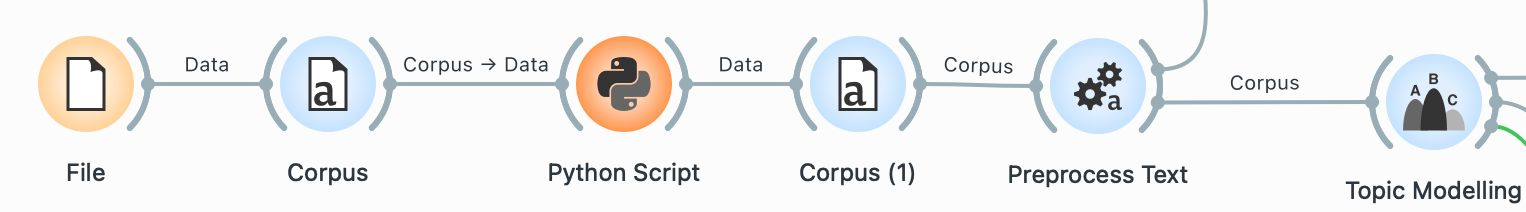
\includegraphics[width=\linewidth]{../odm_screenshots/week10.png}
  \end{center}

  \vspace{0.4em}
  \begin{center}
    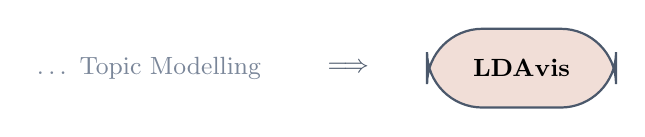
\begin{tikzpicture}[every node/.style={font=\small}]
      \node[font=\small, text=slatelight] (l) {\ldots\ Topic Modelling};
      \node[font=\small, text=slate, right=0.6cm of l] (arr) {$\Longrightarrow$};
      \node[draw=slate, thick, rounded corners=20pt, fill=corallight,
            minimum width=2.4cm, minimum height=1.0cm, right=0.6cm of arr]
            (ldavis) {\textbf{LDAvis}};
    \end{tikzpicture}
  \end{center}
\end{frame}

\begin{frame}{Nouns Only for Topic Modeling}{Why our preprocessing differs from Week 9}
  Week 9 sentiment kept \textbf{nouns, verbs, and adjectives}, because feeling lives in verbs and adjectives too.
  For topic modeling we keep \textbf{nouns only}.

  \vspace{0.5em}
  \begin{center}
    \small
    \begin{tabular}{@{}l l l@{}}
      \toprule
      \textbf{POS tag} & \textbf{Meaning}       & \textbf{Example} \\
      \midrule
      NNG              & Common noun (일반명사)   & 독립 \emph{(independence)} \\
      NNP              & Proper noun (고유명사)   & 고구려 \emph{(Goguryeo)} \\
      \bottomrule
    \end{tabular}
  \end{center}

  \vspace{0.6em}
  \begin{callcoral}[Why not verbs?]
    Topics are about \emph{what a text is about}, and in Korean, \emph{what} is carried by nouns.
    Verbs like 하다 (\emph{do}) and 되다 (\emph{become}) appear everywhere; they blur topics rather than separate them.
    Drop them, and the themes sharpen.
  \end{callcoral}
\end{frame}

\begin{frame}{LDAvis: The Interactive View}{A sibling widget in orange3-text, not an add-on you install separately}
  Pipe the \emph{All Topics} output into the \textbf{LDAvis} widget and you get an interactive view of the model.
  \begin{itemize}
    \item \textbf{Map} on the left: each circle is a topic, circle size is prevalence, distance is dissimilarity.
    \item \textbf{Bar chart} on the right: red = how often the word appears in the selected topic, grey = how often across the whole corpus.
    \item \textbf{$\lambda$ slider} blends raw frequency ($\lambda = 1$) with distinctiveness ($\lambda = 0$).
  \end{itemize}

  \vspace{0.4em}
  \begin{callblue}[Practical tip]
    At $\lambda = 1$ the top words are whatever is frequent in the topic, which is often the same across topics. At
    $\lambda \approx 0.2$--$0.35$ you see the words that make each topic \emph{distinctive}. Start at $0.3$.
  \end{callblue}
\end{frame}

% ==================================================================
\section{Application: The NIKH Corpus}

\begin{frame}{The NIKH Corpus}{Korean history textbooks from three political eras}
  The National Institute of Korean History corpus (\emph{국사편찬위원회}) collects
  Korean history textbooks spanning 1895--2016. For today's demo we use the
  \textbf{11-book clustering sample} already on the course website.

  \vspace{0.5em}
  \begin{center}
    \small
    \begin{tabular}{@{}l c l@{}}
      \toprule
      \textbf{Era}                 & \textbf{Books} & \textbf{Examples}                                       \\
      \midrule
      Colonial (1940)               & 3              & 심상소학국사보충아동용 1--2; 교수참고서                   \\
      Authoritarian (1973--1987)    & 4              & 중학교 국사 3차 (1973); 고등학교 국사 4차 (1981); \ldots  \\
      Democratic (1995--2002)       & 4              & 고등학교 국사 6차 (1995); 초등학교 사회 6-1 7차 (2002)     \\
      \bottomrule
    \end{tabular}
  \end{center}

  \vspace{0.5em}
  The corpus is \emph{small in document count} (11) but \emph{large in prose}
  (tens to hundreds of thousands of characters per book). That is exactly the
  shape of corpus LDA was designed for.
\end{frame}

\begin{frame}{Research Questions for the Demo}{What we will ask of the NIKH corpus in class}
  \begin{enumerate}
    \item What themes run through Korean history textbooks as a group?
    \item Do Colonial-era textbooks emphasise different topics than post-1987 Democratic-era ones?
    \item Is there a topic that is more prominent in elementary versus high-school textbooks?
    \item Are some topics near-universal (every textbook uses them) and others era-specific?
  \end{enumerate}

  \vspace{0.6em}
  \begin{callcoral}[A research choice, not a given]
    The \texttt{era} labels (Colonial / Authoritarian / Democratic) are an \emph{editorial} split
    from the corpus metadata. Different historians might draw the lines differently.
    The periodisation is part of your analysis, not a fact handed to you by the algorithm.
  \end{callcoral}
\end{frame}

\begin{frame}{What to Expect in the Demo Output}{Plausible topics for an LDA with $k=4$ on this corpus}
  \begin{center}
    \small
    \begin{tabular}{@{}l l l@{}}
      \toprule
      \textbf{Topic} & \textbf{Likely top words}                    & \textbf{Our working label} \\
      \midrule
      T1 & 고구려, 백제, 신라, 삼국, 왕조, 시대      & Ancient \& pre-modern states \\
      T2 & 조선, 왕, 시대, 성리학, 문화             & Joseon dynasty \\
      T3 & 일제, 독립, 운동, 저항, 식민, 항일        & Colonial / resistance \\
      T4 & 민주, 경제, 산업화, 발전, 정부, 국민      & Modern Korea \\
      \bottomrule
    \end{tabular}
  \end{center}

  \vspace{0.6em}
  What we \emph{expect} to see in the document--topic table:
  \begin{itemize}
    \item 1940 textbooks skewed toward T1--T2 (the Japanese colonial authorities taught a ``pre-modern'' Korea).
    \item 1980s textbooks mixing T3 strongly (the colonial period \emph{as} a topic).
    \item 2002 textbooks spreading weight across T1--T4 (broadest coverage).
  \end{itemize}
\end{frame}

% ==================================================================
\section{Interpreting Topics Responsibly}

\begin{frame}{Strengths of LDA}{What the method is good for}
  \begin{itemize}
    \item \textbf{Exploratory.} Reveals structure in corpora too large to close-read.
    \item \textbf{Mixture-aware.} A textbook can be 60\% colonial-era and 40\% modernisation; clustering could not say that.
    \item \textbf{Comparative.} Topic weights are numbers: you can group by era, decade, author, level.
    \item \textbf{Portable.} The same widget works on tweets, speeches, newspaper articles, or textbook chapters.
  \end{itemize}
\end{frame}

\begin{frame}{Limitations of LDA}{What the method will \emph{not} do for you}
  \begin{itemize}
    \item \textbf{Topics are statistical, not semantic.} They are co-occurrence patterns; \emph{you} give them names.
    \item \textbf{Sensitive to preprocessing.} Change stopwords, POS filter, or document length: topics change.
    \item \textbf{Sensitive to $k$.} Re-running with $k=3$ vs $k=7$ gives different themes.
    \item \textbf{Non-deterministic.} Two runs with the same $k$ can produce different topic orderings (and sometimes different topics).
    \item \textbf{Junk topics happen.} Expect one or two topics to be incoherent at any given $k$.
  \end{itemize}

  \vspace{0.3em}
  \begin{callcoral}[A useful reminder]
    Grimmer, Roberts \& Stewart: \emph{``All quantitative models of language are wrong, but some are useful.''}
    LDA is a \textbf{reading aid}, not an oracle.
  \end{callcoral}
\end{frame}

\begin{frame}{Best Practices for Interpretation}{The checklist we will use in the demo}
  \begin{enumerate}
    \item Run LDA twice with the same $k$. Are the topics stable? If not, raise or lower $k$.
    \item For each topic, read the \textbf{top 10--15 words}. Draft a label that covers most of them.
    \item Open the \emph{Corpus} output and find the 2--3 books with the \textbf{highest weight} for each topic. Does the book title fit your label?
    \item Look for \textbf{one ``junk'' topic} and be honest about it.
    \item Compare topic weights across \texttt{era}. A \emph{Box Plot} grouped by era is usually enough.
  \end{enumerate}
\end{frame}

% ==================================================================
\section{Looking Ahead}

\begin{frame}{For the Lab}{Interactive, workflow, short write-up}
  \textbf{Explore.} Work through the NIKH clustering interactive on the course website. Note which books cluster together,
  and hold that in your head while you run LDA.

  \vspace{0.4em}
  \textbf{Build.} The 5-widget Orange pipeline on \texttt{nikh\_clustering\_demo.csv}:
  Corpus $\to$ Preprocess $\to$ Python Script (Kiwi, nouns only) $\to$ Topic Modelling (LDA, $k=4$) $\to$ Word Cloud.

  \vspace{0.4em}
  \textbf{Write.} 3--4 sentences per topic:
  \begin{itemize}
    \item your label for the topic;
    \item the top 5 words that earned that label;
    \item which era(s) use it most, read off the \emph{Corpus} output.
  \end{itemize}
\end{frame}

\begin{frame}{Where This Leaves Us}{A map of the semester so far}
  \begin{center}
    \small
    \begin{tabular}{@{}l l l@{}}
      \toprule
      \textbf{Week} & \textbf{Method}                    & \textbf{What it gives you} \\
      \midrule
      4--5 & BoW / TF--IDF                              & descriptive word frequencies \\
      7    & Clustering (K-means, hierarchical)         & one group per document \\
      8    & Word embeddings                            & meaning as vectors \\
      9    & Dictionary sentiment                       & a tone score per document \\
      \textbf{10} & \textbf{LDA topic modeling}        & \textbf{a theme mixture per document} \\
      \bottomrule
    \end{tabular}
  \end{center}

  \vspace{0.6em}
  \textbf{Recommended reading.} Grimmer, Roberts \& Stewart, Chapter 13: \emph{Topic Models}.
\end{frame}

\begin{frame}{Week 11: Final Review \& Assessment}{May 11 --- covering Weeks 7--10}
  \textbf{On the day:}
  \begin{itemize}
    \item \textbf{10-question assessment} via Qualtrics (same platform as the midterm).
    \item \textbf{Application exercise.} Apply \emph{one} of the methods you have learned ---
      clustering, word embeddings, sentiment, or LDA --- to a question I will pose,
      using a dataset I will provide on the day.
    \item Come prepared to use \emph{any} of them. You will pick your method once you see the task.
    \item Followed by a review of the term and a look ahead to the Research Methods Project.
  \end{itemize}

  \vspace{0.4em}
  \begin{callblue}[Between today and May 11]
    We do not meet. I will email you more information about the Research Methods Project in the meantime.
  \end{callblue}
\end{frame}

\begin{frame}{Week 12: Research Methods Project Workshop}{May 18 --- our last meeting}
  A working session for your final paper.
  \begin{itemize}
    \item In-class assistance from me and peer support from your classmates.
    \item Bring whatever you are stuck on: a research question, a dataset, a draft, a half-finished pipeline.
    \item Troubleshoot together, plan the write-up, ask questions.
    \item This is our last chance to come together as a group.
  \end{itemize}

  \vspace{0.4em}
  \begin{callcoral}[What to expect]
    Attendance is expected. The environment is supportive --- not an assessment. Come prepared to work on
    your project and to help a classmate with theirs.
  \end{callcoral}
\end{frame}

% ==================================================================
\appendix
\section{Appendix: Other Topic Modeling Methods}

\begin{frame}{Appendix: Other Topic Modeling Methods}{LSI, HDP, NMF --- three alternatives you may see in the literature}
  \begin{center}
    \small
    \begin{tabular}{@{}l l l@{}}
      \toprule
      \textbf{Method} & \textbf{How it works}                                  & \textbf{When useful} \\
      \midrule
      LSI & A linear-algebra trick (SVD) on the term--document matrix.       & Search and information retrieval; \\
          & Produces ``latent dimensions,'' not probability distributions.    & fast, but topics are hard to read. \\[0.4em]
      NMF & Factorises the (non-negative) term--document matrix into          & Often produces sharper, more \\
          & a word part and a document part. Not probabilistic, but           & coherent topics than LDA; \\
          & topics often look clean.                                          & common in recent NLP work. \\[0.4em]
      HDP & A non-parametric cousin of LDA: you don't pick $k$ ---             & When you genuinely don't know \\
          & the model infers the number of topics from the data.              & how many topics to ask for. \\
      \bottomrule
    \end{tabular}
  \end{center}

  \vspace{0.6em}
  All three are available in Orange's Topic Modelling widget. We stay with LDA in this course because it
  produces probability mixtures that are easy to teach and because you pick $k$ deliberately.
\end{frame}

\begin{frame}{Appendix: Quick Comparison}{How each method answers the same two questions LDA answers}
  \begin{center}
    \small
    \begin{tabular}{@{}l c c c@{}}
      \toprule
                                & \textbf{LDA} & \textbf{LSI} & \textbf{NMF} \\
      \midrule
      Probabilistic?            & yes          & no           & no           \\
      Output: topic--word       & $\phi_k(w)$, probabilities & loadings & non-negative weights \\
      Output: doc--topic        & $\theta_d(k)$, mixture    & coordinates & non-negative weights \\
      You choose $k$?           & yes          & yes          & yes          \\
      \bottomrule
    \end{tabular}
  \end{center}

  \vspace{0.5em}
  \textbf{HDP} sits outside this table because $k$ is inferred rather than chosen. Its output is still a topic mixture per document, like LDA.

  \vspace{0.4em}
  \textbf{Practical advice.} If LDA gives you incoherent topics no matter what $k$ you choose, NMF is the
  obvious next thing to try. It uses the same preprocessing pipeline.
\end{frame}

\end{document}

